\documentclass{beamer}
%% Possible paper sizes: a0, a0b, a1, a2, a3, a4.
%% Possible orientations: portrait, landscape
%% Font sizes can be changed using the scale option.
\usepackage[size=a0,orientation=portrait,scale=1.8]{beamerposter}
\usetheme{LLT-poster}
% \usecolortheme{ComingClean}
\usecolortheme{Entrepreneur}
% \usecolortheme{ConspiciousCreep}  %% VERY garish.

\usepackage[utf8]{inputenc}
\usepackage[T1]{fontenc}
\usepackage{libertine}
\usepackage[scaled=0.92]{inconsolata}
\usepackage[libertine]{newtxmath}

\usepackage{mwe}
\usepackage{pifont} % pro pekne znacky http://ctan.org/pkg/pifont
\newcommand{\cmark}{\ding{51}} % pekne znacky
\newcommand{\xmark}{\ding{55}} % pekne zncky§

% \usebackgroundtemplate{\tikz\node[opacity=0.1]{\includegraphics[width=\paperwidth,height=\paperheight]{./Pics/world.png}};}

% \title{\raisebox{\heightof{B)}-\height+7mm}{\includegraphics[height=1.3em]{img/beacon-network-short.png}}\#filterbubble}
\title{\#filterbubble}
\author[dostal.jakub@outlook.com]{F. Sandroni, J. Dostal}
% Optional foot image
% \footimage{\includegraphics[width=2.1em]{img/ga4gh.png}}


\begin{document}
\begin{frame}[fragile]
\begin{columns}[T]
% #############################################################################
% #############################################################################
% #############################################################################
% First Column
\begin{column}{.33\textwidth}

\begin{block}{Filter Bubble}
    \center
    \begin{large}\textbf{Living in one's own information environment.}\end{large}
    \vspace{0.8cm}
    \begin{itemize}
        \item occures on social networks
        \item caused by preferential algorithms
        \item first mentioned by Eli Pariser (2011)
    \end{itemize}
\end{block}
% #############################################################################
\begin{block}{Twitter}
	\begin{itemize}
		\item microblogging platform
        \item \textbf{following, followers} system
		\item Twitter API is suitable data source
	\end{itemize}
	\center
	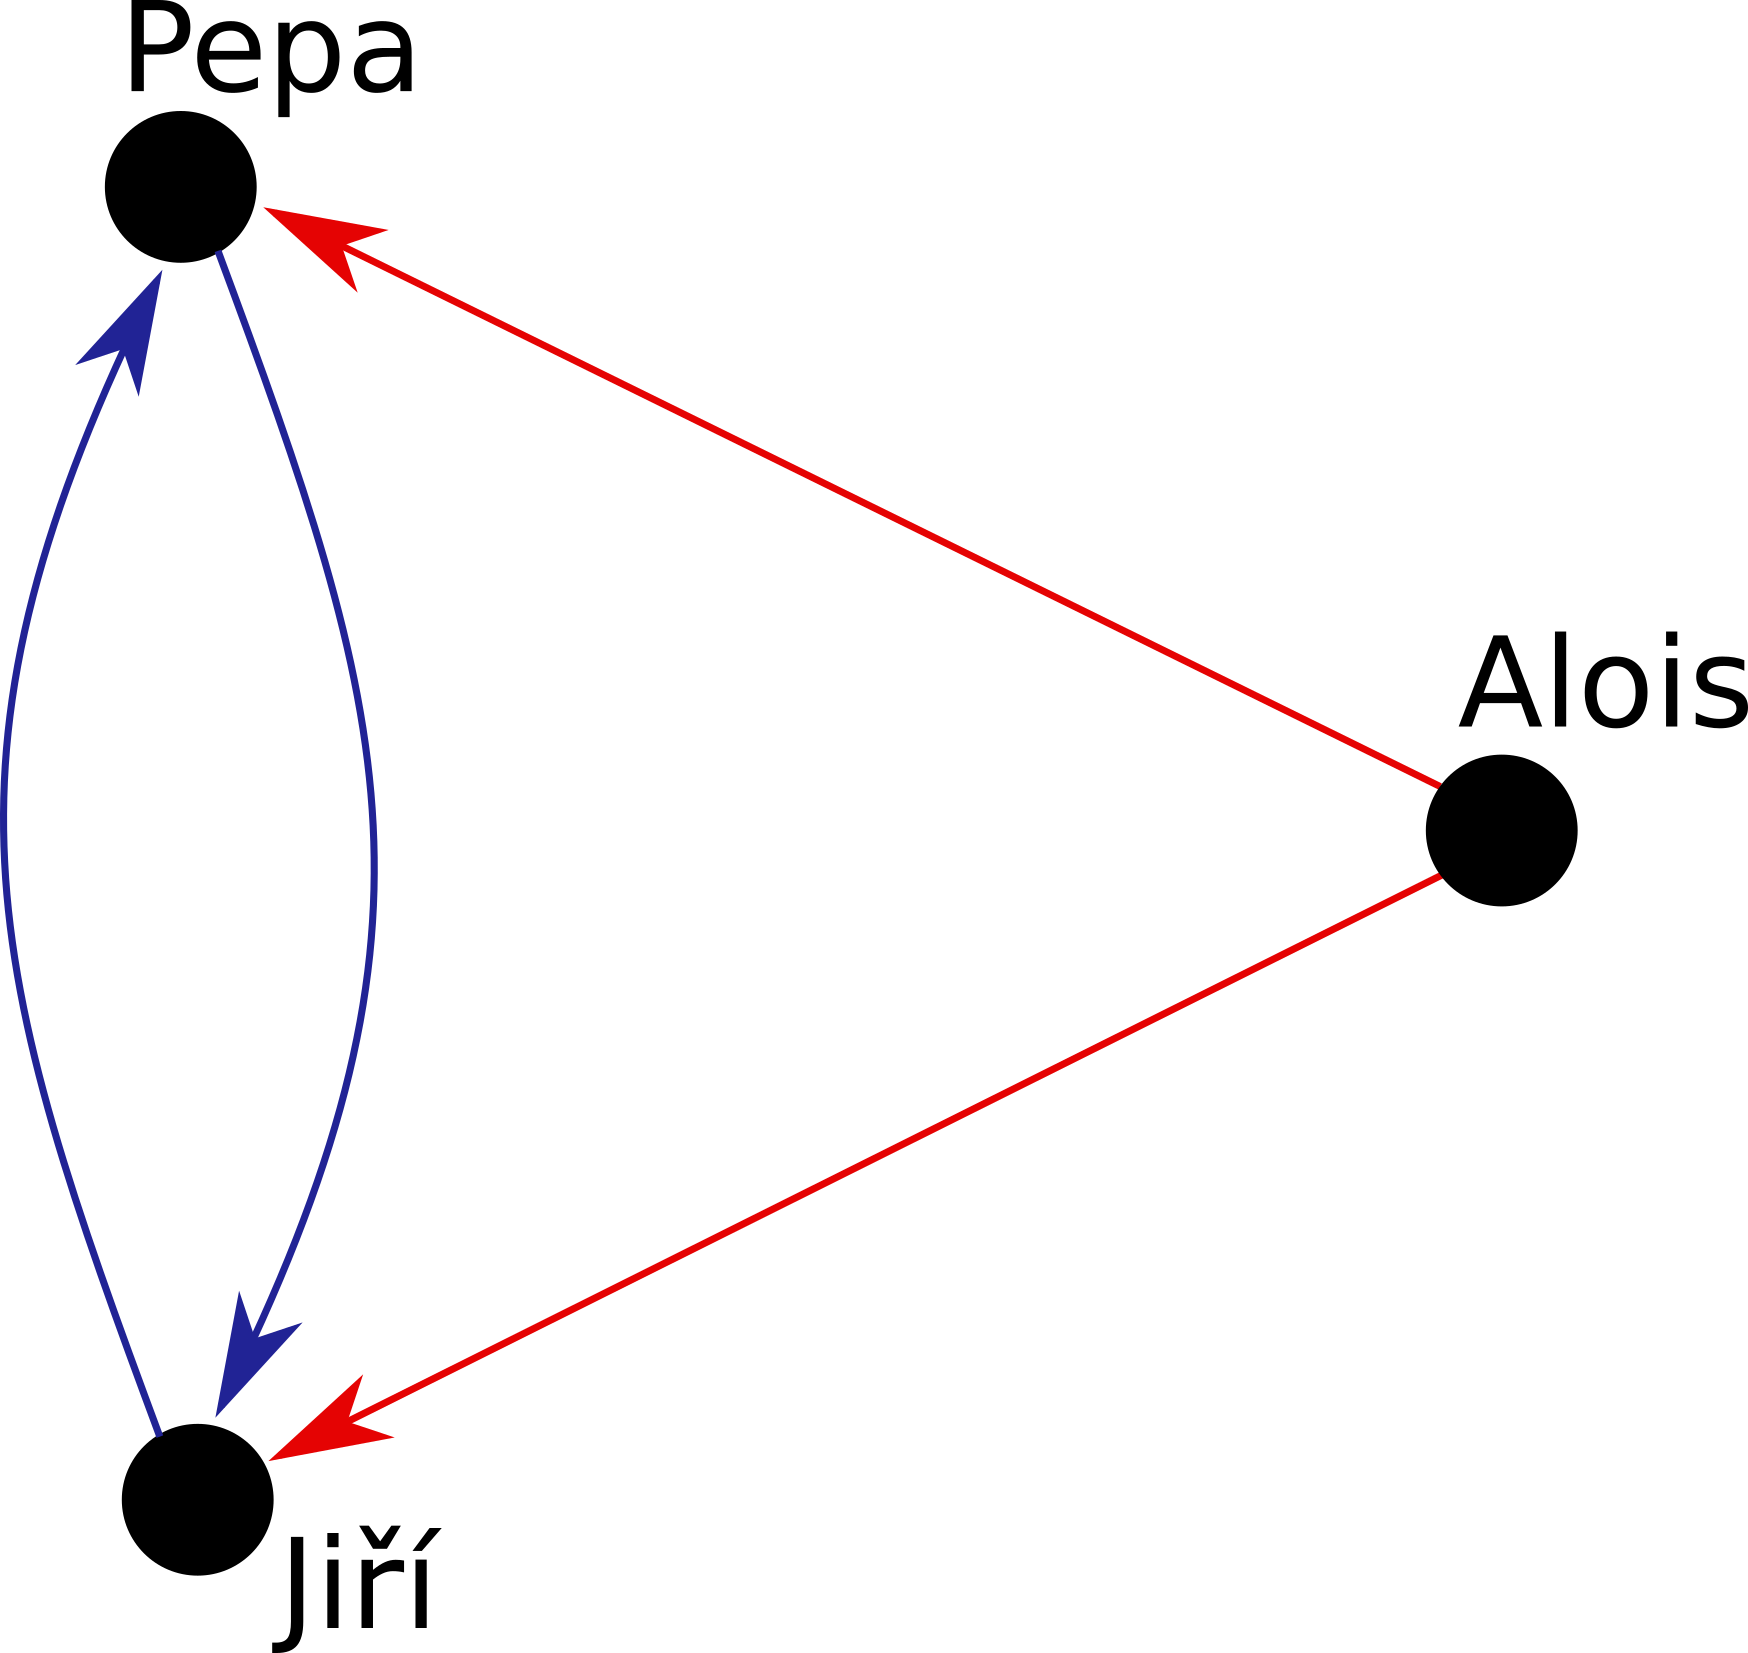
\includegraphics[scale=0.55]{./Pics/pepa.png}
\end{block}
% #############################################################################
\begin{block}{Studied groups selection}
    \begin{columns}
        \begin{column}{.5\textwidth}
            \begin{itemize}
                \item random sample from followers of the significant group
            \end{itemize}
        \end{column}
        \begin{column}{.5\textwidth}
            \center
            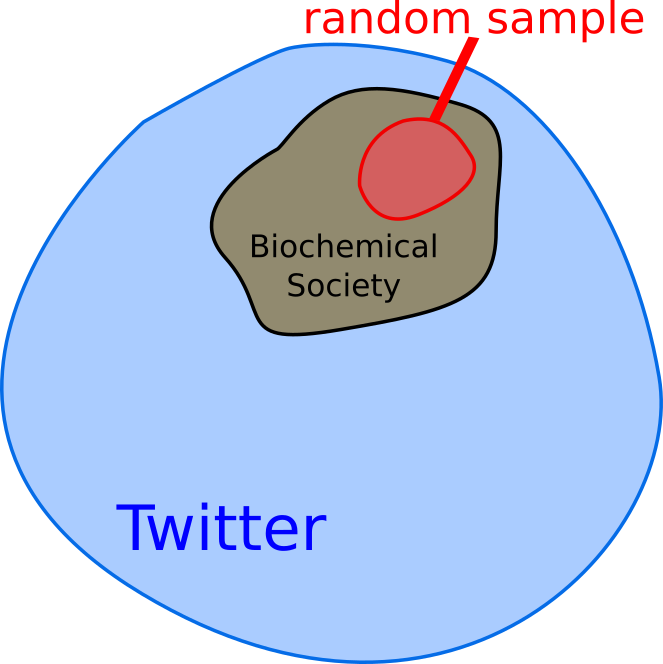
\includegraphics[scale=0.45]{./Pics/sets.png}
        \end{column}
    \end{columns}
    \center
    $\text{Twitter} \rightarrow \text{Biochemical Society} \rightarrow \text{\textbf{studied people}}$
\end{block}
% #############################################################################
\begin{block}{Tweets collection}
    \begin{columns}
    \column{.5\textwidth}
    	\begin{itemize}
            \item analysing content affecting the studied people
    	\end{itemize}
    \column{.5\textwidth}
    	\center
    	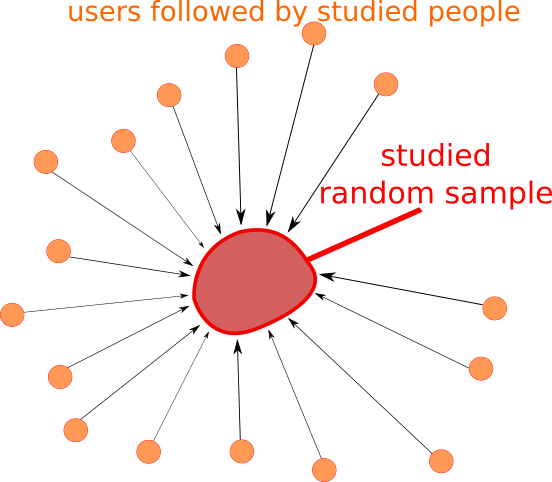
\includegraphics[scale=0.65]{./Pics/followers.png}
    \end{columns}
    \vspace{0.8cm}
    \begin{itemize}
        \item i. e. content from \textbf{followed people}
    \end{itemize}
\end{block}
% #############################################################################
\begin{block}{Tweets filtering}
\begin{itemize}
    \item filter only tweets on given topic
\end{itemize}
\vspace{0.3cm}
Keyword \textbf{"Trump"}:
\vspace{0.7cm}
\begin{itemize}\centering
    \item[\textcolor{black}{\xmark}] I had fish and chips for lunch.
    \item[\textcolor{black}{\cmark}] I'm glad Donald \textbf{Trump} is the president of the USA.
    % \item[\textcolor{black}{\xmark}] The president of the USA is a gentleman.
\end{itemize}
\end{block}
% #############################################################################
\begin{block}{Sentimental analysis}
\begin{itemize}
    \item measure sentiment of collected tweets
    \item \textbf{positive} vs. \textbf{negative} tweets
\end{itemize}
\center
\textit{Donald Trump is a terrible person.}\\
\textbf{(0.14)}\\
\vspace{0.5cm}
\textit{Donald Trump is a great person.}\\
\textbf{(0.95)}
\end{block}

\end{column}
% #############################################################################
% #############################################################################
% #############################################################################
% Second Column
\begin{column}{.63\textwidth}

\begin{customalertblock}{Motivation}
    \begin{columns}
        \begin{column}{.5\textwidth}
            \begin{large}\textbf{Threats for democracy:}\end{large}
            \vspace{0.5cm}
            \center
            content \textbf{homogeneity}\\
            $\Downarrow$\\
            loss of objectivity\\
            $\Downarrow$\\
            \textbf{radicalization}
        \end{column}
        \begin{column}{.5\textwidth}
            \begin{large}\textbf{Goals:}\end{large}
            \vspace{0.5cm}
            \begin{itemize}
                \item filter bubble detection
                \item filter bubble quantification
            \end{itemize}
        \end{column}
    \end{columns}
\end{customalertblock}
% #############################################################################
\begin{columns}
    \column{0.5\textwidth}
        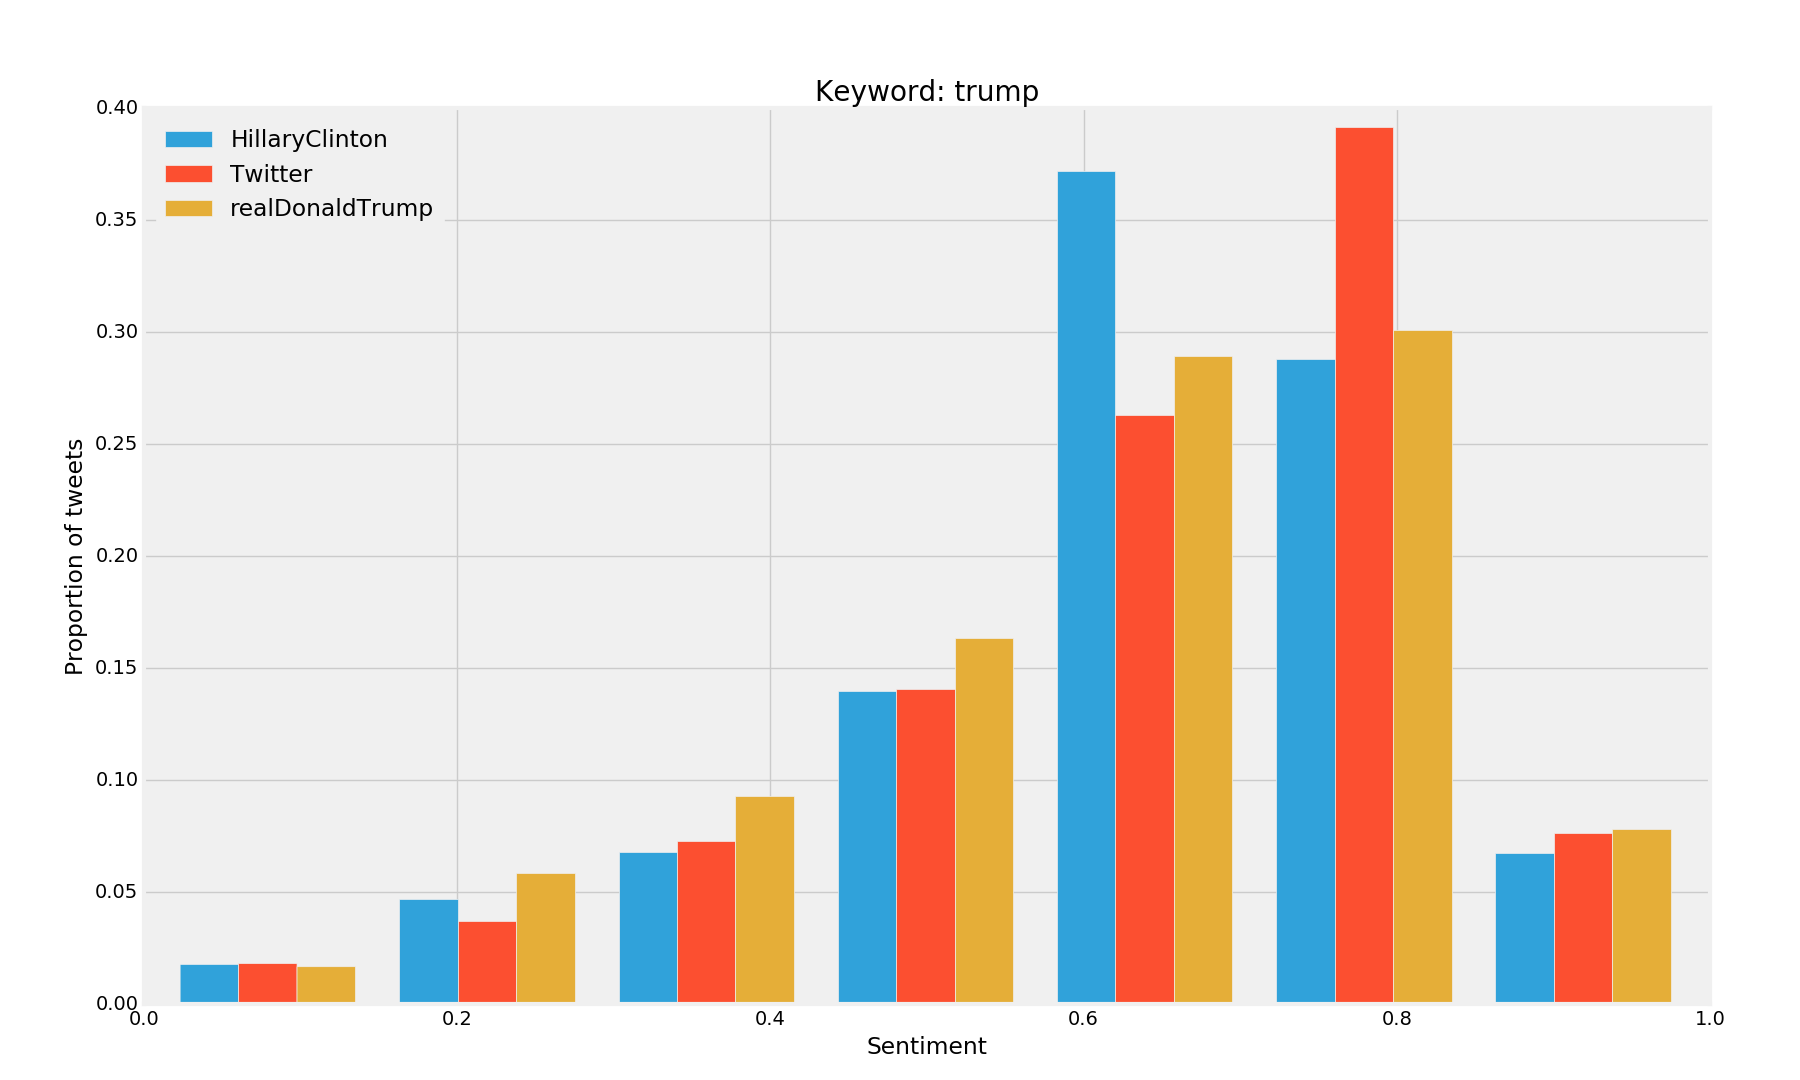
\includegraphics[scale=0.585]{./Pics/hist-trump.png}
    \column{0.5\textwidth}
        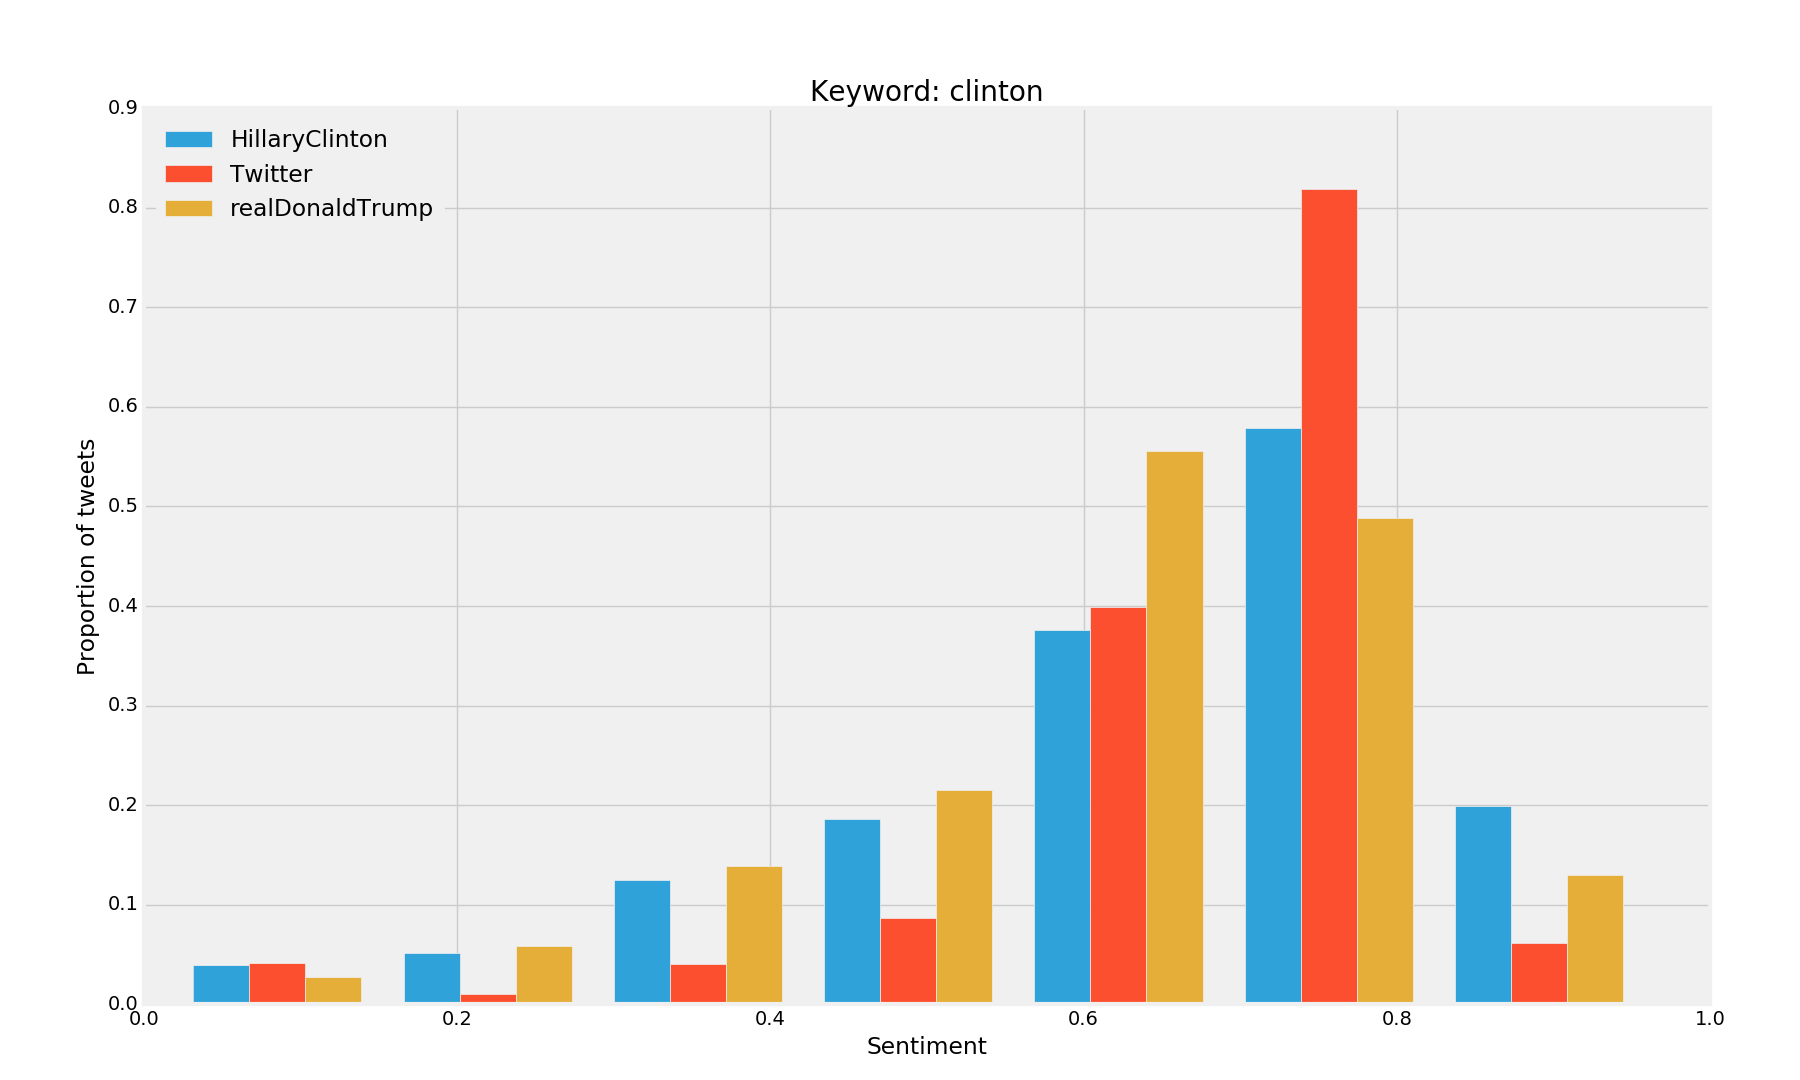
\includegraphics[scale=0.585]{./Pics/hist-clinton.png}
\end{columns}
% #############################################################################









\end{column}
\end{columns}
% #############################################################################
% #############################################################################
% #############################################################################
\end{frame}
\end{document}
